\documentclass[12pt]{article}
\usepackage{listings}
\usepackage{amsmath}
\usepackage{graphicx} % for including gif

% The following nonsense is coloring for code samples %%%%%%%
\usepackage{color}

\definecolor{codegreen}{rgb}{0,0.6,0}
\definecolor{codegray}{rgb}{0.5,0.5,0.5}
\definecolor{codepurple}{rgb}{0.58,0,0.82}
\definecolor{backcolour}{rgb}{0.95,0.95,0.92}

\lstdefinestyle{mystyle}{
	backgroundcolor=\color{backcolour},   
	commentstyle=\color{codegreen},
	keywordstyle=\color{magenta},
	numberstyle=\tiny\color{codegray},
	stringstyle=\color{codepurple},
%	basicstyle=\footnotesize,
	breakatwhitespace=false,         
	breaklines=true,                 
	captionpos=b,                    
	keepspaces=true,                 
	numbers=left,                    
	numbersep=5pt,                  
	showspaces=false,                
	showstringspaces=false,
	showtabs=false,                  
	tabsize=2
}

\lstset{style=mystyle}
%%%%%%%%%%%%%%%%%%%%%%%%%end nonsense%%%%%%%%%%%%%%%%%%%%%%%%%%%%%%%%%%%%%%

\begin{document}

\title{IS\&T 5420 Homework 1}
\author{Benjamin Paul Suntrup}
\maketitle
	
\section*{Problem 1}
\begin{itemize}
	\item $P_t$ is the amount of principal in the account at time $t$. $t$ ranges over the reals.
	\item $P_0$ is the initial principal in the account. $P_0$ ranges over the reals.
	\item $m$ is the number of times the interest is compounded per year. $m$ must be positive.
	\item $j$ is the annual interest rate. One would think that interest must be positive. The recent financial history of the European Union shows that $j$ ranges over the reals.
	\item $t$ is the time in years that the account has been growing. $t$ ranges over the reals.
\end{itemize}

\section*{Problem 2}
I asked in class if you meant that the interest is compounded monthly or yearly here, and you answered yearly. So I proceed to answer accordingly.

$$P_5 = \$1000(1+\frac{0.015}{1})^{5\times 1} = \$1077.28$$

\section*{Problem 3}
\begin{itemize}
	\item $P_5 = \$1000(1+\frac{0.015}{2})^{5\times 2} = \$1077.58$
	\item $P_5 = \$1000(1+\frac{0.015}{4})^{5\times 4} = \$1077.73$
	\item $P_5 = \$1000(1+\frac{0.015}{6})^{5\times 6} = \$1077.78$
	\item $P_5 = \$1000(1+\frac{0.015}{12})^{5\times 12} = \$1077.83$
\end{itemize}

As the frequency with which the interest compounds increases, the total value of the account goes up over the same time period.

\section*{Problem 4}




\begin{center}
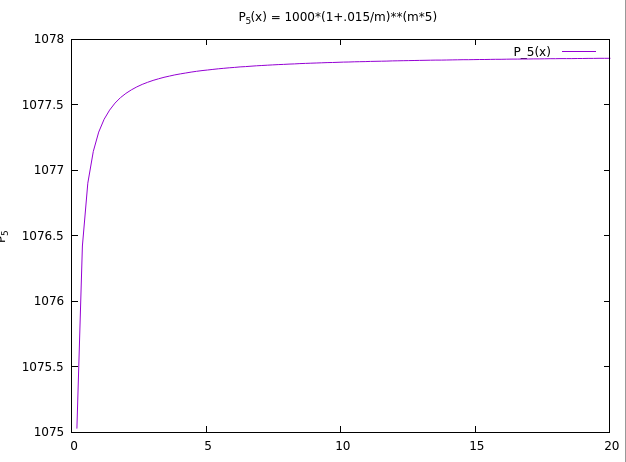
\includegraphics[scale=0.5]{screenshot1.png}
\end{center}

\section*{Problems 5}
\begin{lstlisting}[language=python, caption=$P_t$ calculator]
#!/usr/bin/python3.5
P_0 = 1000
t = 5

# iterate over values of m, and print corresponding P_t
for j in [.015,.025,.05,.075,.1]:
	for m in [2,4,6,12]:
		P_t = P_0*(1+j/m)**(t*m)
		print("j={}, m={} => P_t={}".format(j,m,P_t))
\end{lstlisting}

\begin{lstlisting}[caption=$P_t$ at different values of $m$ and $j$: Output]
j=0.015, m=2 => P_t=1077.58254547074
j=0.015, m=4 => P_t=1077.7329619111877
j=0.015, m=6 => P_t=1077.7832720706283
j=0.015, m=12 => P_t=1077.8336683126824
j=0.025, m=2 => P_t=1132.2708296642568
j=0.025, m=4 => P_t=1132.7077383929188
j=0.025, m=6 => P_t=1132.8542176747685
j=0.025, m=12 => P_t=1133.0011218785867
j=0.05, m=2 => P_t=1280.0845441963565
j=0.05, m=4 => P_t=1282.0372317085844
j=0.05, m=6 => P_t=1282.695963499763
j=0.05, m=12 => P_t=1283.3586785035118
j=0.075, m=2 => P_t=1445.0439426308374
j=0.075, m=4 => P_t=1449.9480257195419
j=0.075, m=6 => P_t=1451.6133600071457
j=0.075, m=12 => P_t=1453.2944082765023
j=0.1, m=2 => P_t=1628.894626777442
j=0.1, m=4 => P_t=1638.6164402903942
j=0.1, m=6 => P_t=1641.9409670661782
j=0.1, m=12 => P_t=1645.3089347785854

\end{lstlisting}

Discussion below, in Problem 6.

\section*{Problems 6}

Below, I've plotted the size of an account after 5 years in dollars with an initial
 deposit of \$1000, an annual interest of $j$ compounded $m$ times per year.
 
 It's interesting to note that as $m$ increases, the value of the account seems to 
 approach the continuous compounding amount. Also, $j$ increases the value of the account
 exponentially.
 
\begin{center}
	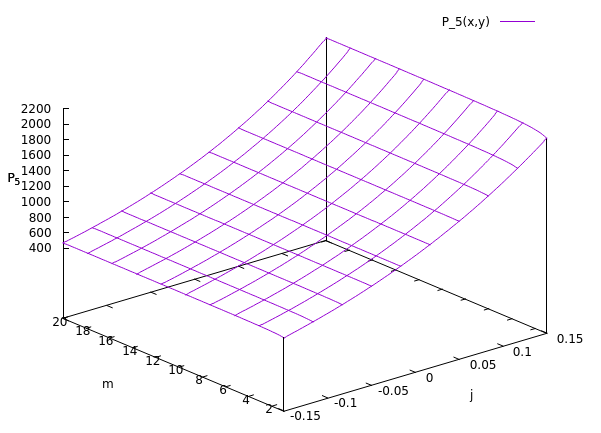
\includegraphics[scale=0.5]{screenshot2.png}
\end{center}

\section*{Problem 8}
Call $f(j) \equiv P_t(j) = P_0(1+\frac{j}{m})^{mt}$. Then 

\newcommand{\dv}[1]{\frac{d}{d#1}}

$$\dv j ln(f(j))=\frac{1}{f(j)}\cdot f'(j)$$

$$\Rightarrow \dv j f(j) = f(j)\cdot \dv{j}ln(f(j))$$

So, we have that

\begin{align*}
\dv j ln(f(j)) &= \dv j ln(P_0(1+\frac{j}{m})^{mt}) \\
	&= mt \dv j [ln P_0 + ln\frac{j}{m}] \\
	&= mt\dv j[ln\; j - ln\; m]\\
	&= mt\dv j ln\; j\\
	&= \frac{mt}{j}
\end{align*}

Hence, $\dv j f(j) = f(j)\cdot \dv j ln\; f(j) = P_0(1+\frac{j}{m})^{mt}\cdot \frac{mt}{j}$

Thus, you would expect an increase in $j$ by $\Delta j$ to
bear about an increase of $\Delta j\cdot P_0(1+\frac{j}{m})^{mt}\cdot \frac{mt}{j}$ in $P_t$.

\section*{Problem 9}
We have

\begin{align*}
1000e^{rt} &= 1000\cdot(1+\frac{0.015}{12})^{12t} \\
\Rightarrow e^{rt} &= 1.00125^{12t} \\
\Rightarrow rt &= 12t\cdot ln\; 1.00125 \\
\Rightarrow r &= 12\cdot ln\;1.00125\approx 0.01499
\end{align*}

\section*{Problem 10}

\begin{align*}
&P_0e^{rt} = P_0(1+\frac{j}{m})^{mt} \\
\Rightarrow\; &e^{rt} = (1+\frac{j}{m})^{mt} \\
\Rightarrow\; &rt = mt\,ln(1+\frac{j}{m}) \\
\Rightarrow\; &r = m\,ln(1+\frac{j}{m})
\end{align*}


\end{document}